\documentclass[12pt]{article}
\usepackage[utf8]{inputenc}
\usepackage[margin=1.5cm]{geometry}
\usepackage{amsmath}
\usepackage{amssymb}
\usepackage{graphicx}
\usepackage{mathtools}
\DeclarePairedDelimiter{\abs}{\lvert}{\rvert}

\begin{document}

\section*{LEZIONE 12}
\subsection*{RICOSTRUZIONE DI FUNZIONI DA DATI DISCRETI, INTERPOLAZIONE POLINOMIALE, ESISTENZA E UNICITÀ, IL PROBLEMA DELLA CONVERGENZA, ESEMPIO DI RUNGE}

In questa lezione cominceremo ad occuparci di un argomento molto importante del calcolo numerico dal punto di vista applicativo, ovvero della \underline{ricostruzione (approssimata) di funzioni da dati discreti}, cioè tramite un \underline{campionamento finito}.\\
In particolare, ci concentreremo su 2 tecniche: l'INTERPOLAZIONE (polinomiale e polinomiale "a tratti") e l'APPROSSIMAZIONE AI MINIMI QUADRATI (di tipo polinomiale).\\
Basti ricordare che le varie tecniche di interpolazione e approssimazione di dati e funzioni sono alla base di molti metodi di enorme interesse applicativo, ad esempio: \underline{grafica} (CAGD), elaborazione di \underline{segnali} e \underline{immagini}, \underline{data science} (machine learning, data mining, $\dotsc$), \underline{discretizzazione} di \underline{modelli differenziali} delle scienze e della tecnologia (\underline{modellistica computazionale:} meccanica, fluidodinamica, meteorologia, elettromagnetismo, \dots). \\
La prima tecnica che studieremo (limitandoci a funzioni reali di una variabile) è l'interpolazione: dati $n+1$ punti $\left\{ (x_i, y_i) \right\}$ con $y_i=f(x_i)$, $0 \leq i \leq n$, sul grafico di una funzione $f:[a,b] \rightarrow \mathbb{R}$, cerchiamo una funzione $f_n \in \mathcal{F}_n$ (dove $\mathcal{F}_n$ è una opportuna famiglia di funzioni "semplici"), tale che
\[
    f_n(x_i) = y_i, \ 0 \leq i \leq n
\]
cioè tale che il grafico di $f_n$ passi per il grafico di $f$ in corrispondenza delle ascisse di interpolazione $\left\{ x_i \right\}$ (che chiameremo \underline{nodi}, mentre gli $\left\{ y_i \right\}$ sono i valori della funzione campionata)
\begin{center}
    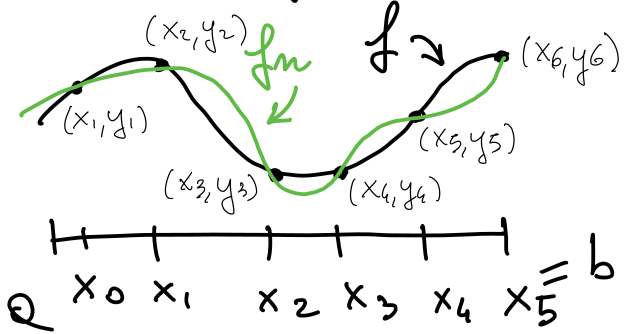
\includegraphics[width=0.45\textwidth]{pag4_img1.png}
\end{center}
Ribadiamo fin da ora che lo scopo dell'interpolazione è di ricostruire (approssimare) la funzione campionata fuori dal campionamento.\\
Quindi $f_n$ andrebbe scelta in modo che 
\[
    dist(f,f_n) \to 0, n \to \infty
\]
dove "dist" è una misura della distanza tra due funzioni, cioè dell'errore che si commette approssimando $f$ con $f_n$. \\
Torneremo più avanti su questo concetto, anticipando che la distanza che useremo è, date $f,g \in C[a,b]$
\[
    \underset{x \in [a,b]}{dist(f,g) = max |f(x) - g(x)|}
\]
cioè il massimo modulo della differenza tra il valore di $f$ e di $g$ al valore di $x$ in $[a,b]$ (osserviamo che per il teorema di Weierstrass sull'$\exists$ di max e min assoluti di una funzione continua, in questo caso $f-g$, su un intervallo chiuso e limitato, questa distanza è ben definita). Naturalmente avrà senso parlare di convergenza solo dopo che avremo scelto quale sia la famiglia di funzioni $\mathcal{F}_n$ e che sia garantita l'$\exists$ di $f_n \in \mathcal{F}_n$ che interpola la funzione campionata $f$. \\
Una scelta naturale (che è stata anche una delle prime storicamente nel XVIII secolo) è $\mathcal{F}_n = \mathbb{P}_n$, cioè i polinomi di grado $\leq n$ (vedremo che il grado è strettamente legato al problema algebrico dell'$\exists$ e unicità dell'interpolazione).\\
Perché i polinomi? Un primo motivo è che i polinomi sono funzioni facili da gestire e memorizzare (un polinomio è completamente determinato dai suoi coefficienti), infatti $p \in \mathbb{P}_n$ ha la forma 
\[
    p(x) = a_0 + a_1x + \dotso + a_nx^n
\]
sono facili da calcolare (visto che il calcolo coinvolge solo operazioni aritmetiche, abbiamo tra l'altro lo schema di H{\"o}rner che minimizza il numero di operazioni), sono facili da derivare e integrare, insomma sono dei buoni "sostituti" di una funzione (purché la stiano approssimando bene). \\
Il problema che dobbiamo risolvere è di tipo algebrico: dati $n+1$ punti del grafico di $f$ cioè $n+1$ punti del piano $\{(x_i,y_i)\}_{0\leq i\leq n}$ con $y_i=f(x_i)$, esiste un polinomio $f_n\in\mathbb{P}_n$ che interpola $f$? E se esiste, è unico?\\ Innanzitutto osserviamo che le incognite in questo problema non sono le "$x$", visto che i nodi di campionamento $\{x_i\}$ fanno parte dei dati del problema, ma sono gli $n+1$ coefficienti $\{a_j\}$. Quindi cercare un polinomio interpolatore in $\mathbb{P}_n$ è una scelta del tutto sensata, perchè il numero di incognite è uguale al numero di vincoli (i vincoli di interpolazione $f_n(x_i)=y_i$, $0\leq i\leq n$).\\Scrivendo esplicitamente tali vincoli otterremo un sistema di equazioni con tante equazioni quante sono le incognite. Per capirlo, trattiamo il caso in cui $n=5$ (come nel disegno fatto sopra), cioè cerchiamo un polinomio di grado 5
\[
    f_5(x)=a_0+a_1x+a_2x^2+a_3x^3+a_4x^4+a_5x^5
\]
I vincoli di interpolazione sono 
\[
    \begin{cases}
        f_5(x_0)=a_0+a_1x_0+\dotso+a_5x_0^5=y_0\\
        f_5(x_1)=a_0+a_1x_1+\dotso+a_5x_1^5=y_1\\
        f_5(x_2)=a_0+a_1x_2+\dotso+a_5x_2^5=y_2\\
        f_5(x_3)=a_0+a_1x_3+\dotso+a_5x_3^5=y_3\\
        f_5(x_4)=a_0+a_1x_4+\dotso+a_5x_4^5=y_4\\
        f_5(x_5)=a_0+a_1x_5+\dotso+a_5x_5^5=y_5\\
    \end{cases}
\]
che è un sistema \underline{LINEARE} di 6 equazioni nelle 6 incognite $a_0,a_1,\dotso,a_5$\\ 
\underline{Perchè} il sistema è \underline{lineare}? Il motivo è che un polinomio di grado $\leq n$ si scrive come \underline{combinazione lineare} degli $n+1$ monomi $1, x, x^2, \dotso, x^n$. In effetti
\[
\mathbb{P}_n = \left\{p(x) = \sum\limits_{j=0}^n a_j x^j \right\}
\]
è uno spazio vettoriale di dimensione $n+1$, una cui base sono gli $n+1$ monomi $x^j$, $0 \leq j \leq n$ (che i monomi $\{ x^j \}_{0 \leq j \leq n}$ siano linearmente indipendenti viene dal fatto che se $p \in \mathbb{P}_n$ e $p(x) = 0$ $\forall x \Rightarrow a_j = 0$ $\forall j$) perché un polinomio di grado $\leq n$ non identicamente nullo può avere al massimo $n$ zeri reali (ne ha esattamente $n$, in generale complessi, contati con la loro molteplicità).\\
Formalmente si può scrivere
\[
\mathbb{P}_n = < 1, x, x^2, \dotso, x^n >
\]
(dove in generale $< g_1(x), \dotso, g_k(x) >$ indica lo spazio vettoriale generato dalle $k$ funzioni $g_j$, cioè l'insieme di tutte le loro possibili combinazioni lineari) e $dim(\mathbb{P}_n) = n+1$ (la dimensione è il numero di elementi di una base, cioè di generatori linearmente indipendenti).\\
In generale il sistema lineare di interpolazione è
\[
f_n(x_i) = \sum\limits_{j=0}^n a_j x_i^j = y_i \ \ \ 0 \leq i \leq n
\]
cioè è un sistema lineare di $n+1$ equazioni in $n+1$ incognite e può essere scritto in forma compatta come
\[
V\underline{a} = \underline{y}
\]
dove
\[
\underline{a} = 
    \begin{bmatrix}
    a_0 \\ a_1 \\ \vdots \\ a_n
    \end{bmatrix}, \ \
\underline{y} =
    \begin{bmatrix}
    y_0 \\ y_1 \\ \vdots \\ y_n
    \end{bmatrix}
    \in \mathbb{R}^{n+1}
\]
sono rispettivamente il vettore dei coefficienti incogniti e il vettore (termine noto) dei valori campionati, mentre $V = (v_{ij}) = (x_i^j)$, con $0 \leq i,j \leq n$ è la matrice del sistema
\[
V =
    \begin{bmatrix}
    1 & x_0 & x_0^2 & \cdots & x_0^n \\
    1 & x_1 & x_1^2 & \cdots & x_1^n \\
    \vdots & \vdots & \vdots & \ & \vdots \\
    1 & x_n & x_n^2 & \cdots & x_n^n
    \end{bmatrix}
    \in \mathbb{R}^{(n+1) \times (n+1)}
\]
che viene chiamata "matrice di Vandermonde" e dipende solo dai nodi di interpolazione (e dal grado $n$).\\
Si può dimostrare che tale matrice è non singolare se e solo se i nodi sono distinti
\[
det(V) \neq 0 \iff x_i \neq x_j, \ \ i \neq j
\]
(non dimostreremo direttamente "$\Leftarrow$", mentre "$\Rightarrow$" è immediata osservando che se $\exists \ i,j$ tali che $i\neq j$ e $x_i\neq x_j$, allora la matrice avrebbe due righe coincidenti e quindi determinante nullo).\\ 
Quindi vedendo il problema di interpolazione come sistema lineare, se i \underline{nodi} sono \underline{distinti} il sistema ha \underline{soluzione unica}, cioè \underline{$\exists !$} il \underline{polinomio} di grado $\leq n$ \underline{che interpola} gli $n+1$ dati.\\
Dimostreremo questo fatto qui sotto, mostrando con le proprietà dei polinomi che il polinomio interpolatore di grado $\leq n$ su $n+1$ nodi distinti se esiste è necessariamente unico e mostrando che esiste in modo costruttivo, cioè scrivendo tale polinomio in una forma esplicita e specifica (detta forma di Lagrange).
\newline \newline
\fbox{\textbf{UNICITA'}}\\
Supponiamo che $\exists$ due polinomi $p,q \in \mathbb{P}_n$ che interpolano, cioè tali che $p(x_i)=y_i=q(x_i)$, $0\leq i \leq n$.\\ Allora il polinomio $p-q \in \mathbb{P}_n$ (ricordiamo che $\mathbb{P}_n$ è uno spazio vettoriale quindi se
\[
p, q \in \mathbb{P}_n \Rightarrow \alpha p + \beta q \in \mathbb{P}_n \ \
\forall \alpha, \beta \in \mathbb{R})
\]
e si ha
\[
(p-q)(x_i) = p(x_i) - q(x_i) = 0, \ \ 0 \leq i \leq n
\]
cioè $p-q$ avrebbe $n+1$ zeri distinti.\\
Ma per il teorema fondamentale dell'algebra già ricordato sopra, $p-q$ può avere al massimo $n$ zeri distinti, a meno che non sia il polinomio nullo, cioè deve essere
\[
(p-q)(x) = 0 \ \ \forall x \Rightarrow p(x) = q(x) \ \forall x
\]

\fbox{\textbf{ESISTENZA}}\\
Dati gli $n+1$ nodi distinti $\{ x_i \}_{0 \leq i \leq n}$ consideriamo per ogni nodo fissato (cioè per ogni $i$ fissato) il "polinomio elementare di Lagrange" così definito
\[
l_i(x) = \frac{N_i(x)}{N_i(x_i)}
\]
dove
\[
N_i(x) = (x-x_0)(x-x_1) \dotso (x-x_{i-1})(x-x_{i+1}) \dotso (x-x_n) = \prod_{j=0, \ j\neq i}^n (x-x_j)
\]
(nel prodotto viene saltato il termine i-esimo)\\
Osserviamo che $N_i(x) \in \mathbb{P}_n$ è un polinomio di grado effettivo $n$, infatti si ha
\[N_i(x)=x^n+\dotso\]
mentre $N_i(x_i)$ è un numero $\ne 0$.\\
Quindi $l_i(x) \in \mathbb{P}_n$ e ha grado effettivo $n$,
\[l_i(x) = \frac{1}{N_i(x_i)}x^n+\dotso\]
Inoltre
\[l_i(x_k) = \delta_{ik} =
\begin{cases}
0 & i\ne k \\
1 & i=k 
\end{cases}\]
(il cosiddetto "delta di Kronecker"). Infatti
\[l_i(x_i) = \frac{N_i(x_i)}{N_i(x_i)} = 1\]
e per $k\ne i$
\[N_i(x_k) = (x_k-x_0)\dotso \overbrace{(x_k-x_k)}^{=\,0} \dotso (x_k-x_n) = 0\]
cioè $N_i (x_k)$,  $k \neq i$ contiene un fattore nullo che annulla il prodotto.\\
Ad esempio 
\[
N_0 (x) = (x-x_1) \dotso (x-x_n)
\]
e 
\[
N_0(x_1) = 0 = N_0(x_2) = \dotso = N_0(x_n)
\]
allo stesso modo
\[ N_1(x) = (x-x_0)(x-x_2) \dotso (x-x_n) \]
\[ N_1(x_0) = 0 = N_1(x_2) = \dotso = N_1(x_n) \]
\[ \dotso \]
\[ N_n(x) = (x-x_0)(x-x_1) \dotso (x-x_{n-1}) \]
\[ N_n(x_0) = 0 = N_n(x_1) = \dotso = N_n(x_{n-1}) \]
possiamo allora definire
\[ f_n(x) = \prod_n(x) = \sum_{i=0}^n y_i l_i(x) \]
(polinomio interpolatore di Lagrange).\\
È chiaro che $\prod_n(x) \in \mathbb{P}_n$ (essendo combinazione lineare di polinomi di grado $n$, i polinomi elementari di Lagrange).\\
Verifichiamo che interpola
\[
\begin{split}
\prod _n (x_k) & = \sum_{i=0}^n y_i l_i (x_k) \\
& = \sum_{i=0}^n y_i \delta_{ik} \\
& = y_k \ \delta_{kk} \quad \longleftarrow \quad \text{perchè } \delta_{ik}=0, i \ne k\\
& = y_k, \quad 0 \leq k \leq n
\end{split}
\]
Chiameremo $\prod_n(x)$ \underline{il} polinomio interpolatore su $n+1$ nodi distinti ("il" perché è unico) scritto in \underline{forma di Lagrange}.\\\\
Possiamo fare subito la seguente\\
\textbf{OSSERVAZIONE 1 (importante)}\\
Se la funzione che stiamo interpolando è un polinomio in $\mathbb{P}_n$ (cioè di grado $\leq n$), chi è l'interpolatore?\\
L'interpolatore è il polinomio stesso, cioè se $f(x) = p(x) \in \mathbb{P}_n$ allora $\prod_n(x) = p(x)$, perché il polinomio interpolatore è \underline{unico} in $\mathbb{P}_n$ e
$p(x)$ ovviamente interpola se stesso.\\
Questo ci fa capire che un polinomio interpolatore su $n+1$ nodi distinti può avere grado $<n$: ad esempio, se $f(x) = a_1x + a_0$ (cioè $f$ è un polinomio di grado 1), allora $\prod_n(x) = f(x) \ \forall n \ge 1$\\
e allo stesso modo $f(x) = a_2x^2 + a_1x + a_0 \Rightarrow \prod_n(x) = f(x) \ \forall n \ge 2$.\\
In generale se $f(x) \in \mathbb{P}_k$ allora $\prod_n(x) = f(x) \ \forall n \ge k$
\begin{center}
    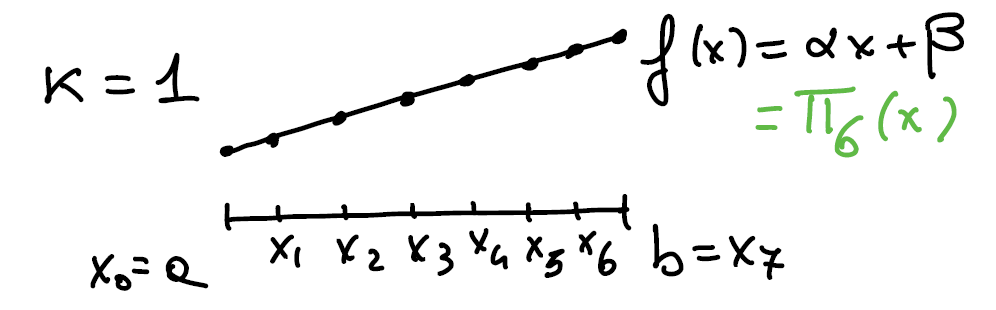
\includegraphics[width=0.6\textwidth]{pag24.PNG}
\end{center}
$\prod_6(x) = f(x) = \alpha x + \beta$ (per quanti modi di campionamento mettiamo, l'interpolatore resterà \underline{sempre} $\alpha x + \beta$ cioè di grado 1).\\\\
\textbf{OSSERVAZIONE 2}\\
dal punto di vista teorico, una volta dimostrata l'unicità avremmo automaticamente
anche l'esistenza e viceversa. Infatti, come abbiamo visto il problema di interpolazione in $\mathbb{P}_n$ su $n+1$ nodi distinti è equivalente al sistema lineare di dimensione $n+1 \ V\underline{a} = \underline{y}$\\
Ora, se c'è unicità $V\underline{a} = \underline{0} \Rightarrow \underline{a} = \underline{0}$ cioè l'applicazione lineare associata a $V$ è \underline{iniettiva} cioè le colonne di $V$ sono linearmente indipendenti cioè $rango(V)=n+1$ e quindi $V$ è invertibile (ricordiamo che $V \underline{a} = \sum_{k=1}^{n+1} a_k l_k(V)$ dove $l_k(V)$ è la colonna $k$-esima di $V$).\\
D'altra parte, se c'è esistenza $\forall \underline{y} \in \mathbb{R}^{n+1}$ significa che le $n+1$ colonne di $V$ generano tutti i vettori di $\mathbb{R}^{n+1}$ cioè sono una base (l'applicazione lineare è \underline{suriettiva}) e quindi $rango(V)=n+1 \Rightarrow V$ invertibile.\\
Però dal punto di vista applicativo non ci accontentiamo di questo, in particolare è stato importante scrivere il polinomio interpolatore $\prod_n$ in una forma esplicita, la forma di Lagrange (ma ce ne sono altre), utile, come vedremo, anche per studiare altri aspetti come ad es. la \underline{stabilità} dell'interpolazione (nel
senso della "risposta" dell'interpolazione ad errori sui valori $\{y_i\}$).\\
Possiamo anche osservare che in base all'Osservazione 1, la forma di Lagrange ci dice che i polinomi elementari di Lagrange
\[\{l_i(x)\}_{0 \le i \le n}\]
sono una base di $\mathbb{P}_n$ (diversa dalla base monomiale $\{x^i\}_{0 \le i \le n}$). \\
Infatti, se $p \in \mathbb{P}_n$ per l'unicità
\[\prod_n(x) = p(x) = \sum_{i=0}^n p(x_i) l_i(x)\]
cioè ogni polinomio di grado $\le n$ si può scrivere come combinazione lineare degli $n+1$ polinomi elementari
(che dipendono \underline{solo} dalla scelta dei nodi di interpolazione $\{x_i\}$)
\newline \newline
\fbox{\textbf{PROBLEMA DELLA CONVERGENZA}}\\
Dopo aver risolto il problema algebrico dell'interpolazione polinomiale (esistenza e unicità del polinomio interpolatore), ci rimane da discutere l'aspetto chiave della convergenza.\\
Lo scopo dell'interpolazione infatti è di usare l'informazione su una funzione ottenuta tramite un campionamento discreto per ricostruire (in modo approssimato)
la funzione su un intero intervallo.\\
L'uso di polinomi per approssimare funzioni ci è familiare con la formula di \underline{Taylor}; tale formula ha però carattere \underline{locale} (tranne che per la classe di funzioni sviluppabili in serie di Taylor, come $e^x,\ \sin{x},\ \cos{x}, \dotso$).\\
Qui invece siamo interessati a un'approssimazione "globale" (su tutto $[a,b]$) e la domanda è: è vero che infittendo il campionamento, la successione $\{\prod_n\}$ dei polinomi interpolatori
approssimerà sempre meglio la funzione campionata? Cioè è vero che $\lim_{n \to \infty} \prod_n = f$? \newline \newline
La possibilità di approssimare bene una funzione continua su un intervallo chiuso e limitato $[a,b]$ tramite un opportuno polinomio è assicurata dal "Teorema di densità di Weierstrass" (che enunciamo solamente, la dimostrazione è molto difficile):
\newline \newline
\textbf{TEOREMA (di densità di Weierstrass)}
\begin{center}
    \fbox{\begin{minipage}[t]{15cm}
        $\forall f \in C[a,b]$ fissata e $\forall \varepsilon > 0$
        \begin{center}
        $\exists \ p_{\varepsilon} \in \mathbb{P}: dist(f,p_{\varepsilon}) \le \varepsilon$
        \end{center}
    \end{minipage}}
\end{center}
Dove:
\begin{itemize}
    \item $\mathbb{P} = \bigcup_{n \ge 0} \mathbb{P}_n$ è l'insieme (che è anche spazio vettoriale) di tutti i polinomi di tutti i gradi
    \item $dist(f,g) = \max_{x\in [a,b]} |f(x)-g(x)|$ è la distanza tra funzioni (continue) che avevamo definito all'inizio
\end{itemize}
Cosa significa in pratica che $dist(f,p_{\varepsilon}) \le \varepsilon$? Per capirlo, osserviamo che avendo una distanza tra funzioni (finora avevamo solo una distanza tra numeri $x,y \in \mathbb{R}$ cioè $|x-y|$) siamo in grado di definire cosa sia un intorno
di raggio $\varepsilon >0$ di una $f\in C[a,b]$
\[I_{\varepsilon}(f) = \{g \in C[a,b] : dist(f,g) \le \varepsilon\}\]
Graficamente, consideriamo un "tubicino" di ampiezza verticale $2\varepsilon$ costruito intorno al grafico di $f$
\begin{center}
    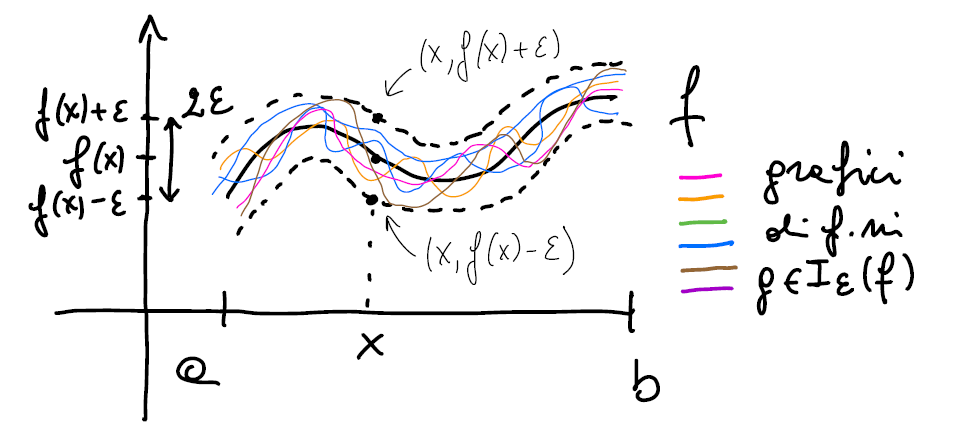
\includegraphics[width=0.8\textwidth]{pag32}
\end{center}
Chi è $I_{\varepsilon}(f)$? \underline{Non} è il "tubicino" dai contorni tratteggiati "paralleli" al grafico di $f$ (questo permette solo
la rappresentazione grafica), invece $I_{\varepsilon}(f)$ è l'insieme delle infinite funzioni continue il cui grafico "vive" nel tubicino, cioè i cui valori $\forall x \in [a,b]$ stanno tra $f(x)-\varepsilon$ e $f(x)+\varepsilon$, cioè 
\[f(x)-\varepsilon \le g(x) \le f(x)+\varepsilon \]
Ma qualsiasi di queste funzioni $g$ sta approssimando $f$ a meno di $\varepsilon$ su \underline{tutto} l'intervallo $[a,b]$.\\
Quindi, cosa ci sta dicendo il teorema di densità di Weierstrass? Che ogni $f \in C[a,b]$ si può \underline{approssimare} \underline{arbitrariamente} bene
su tutto l'intervallo (perchè stiamo parlando del \underline{massimo errore}) con un \underline{opportuno polinomio} (di grado opportuno, che dipenderà da $\varepsilon$ e da $f$).\\
Una conseguenza (che non dimostriamo) del teorema di Weierstrass è che $\forall n\ge0\ \exists$ un (unico) polinomio $p_n^* \in \mathbb{P}_n$ tale che
\[\min_{p \in \mathbb{P}_n} dist(f,p) = dist(f,p_n^*) \underset{n \to \infty}{\longrightarrow} 0\]
che si chiama "polinomio di \underline{migliore approssimazione} uniforme" di $f$ in $\mathbb{P}_n$ (purtroppo questo polinomio ottimale
è molto difficile da calcolare); ma visto che è possibile approssimare bene $f \in C[a,b]$ (e d'ora in poi ci muoveremo nell'ambito di funzioni almeno continue) con polinomi, c'è la speranza che infittendo il campionamento, la successione di interpolatori $\{\prod_n\}$ converga nella distanza del max errore a \\$f \in C[a,b]$? Cioè è vero che $\lim_{n \to \infty} \prod_n = f$ nel senso che $dist(f,\prod_n) \to 0,\ n \to \infty$? (la speranza viene dal fatto che infittendo il campionamento stiamo
in effetti aumentando l'informazione sulla funzione $f$)\\
Purtroppo la risposta è \underline{\underline{NO}}, cioè in generale \underline{non è vero} che la successione di interpolatori converge alla funzione campionata (come vedremo, la convergenza dipende dalla distribuzione dei nodi $\{x_i\}$).\\
A questo proposito, consideriamo uno dei metodi più usuali di campionamento a \underline{passo costante} in $[a,b]$, cioè
\[x_i = a+ih, \quad 0\le i \le n, \quad h = \frac{b-a}{n}\]
che consiste nel partizionare $[a,b]$ in $n$ sottointervalli di ampiezza uguale e prendere come nodi di campionamento i loro estremi
\begin{center}
    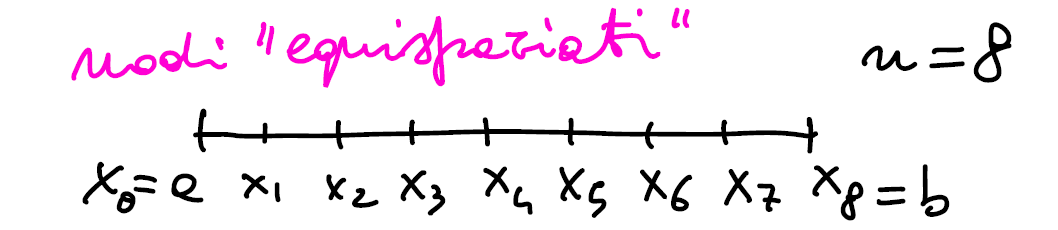
\includegraphics[width=0.6\textwidth]{pag37.PNG}
\end{center}
\[
x_0 = a, x_1 = a+h, x_2 = a+2h, \dotso, x_n = a+nh = b
\]
Questo è un metodo di campionamento del tutto naturale nelle scienze sperimentali e nelle applicazioni tecnologiche, si pensi ad esempio al caso in cui la variabile indipendente è il tempo e si campiona con un passo temporale costante (1 min, 1 sec, 1 millisec, $\dotso$).\\
Bene (anzi, male), purtroppo ci sono funzioni anche molto regolari per cui \underline{l'interpolazione} polinomiale a \underline{passo costante} \underline{non} converge.\\
Un classico esempio (che non possiamo trattare rigorosamente perché dietro c'è un'intera teoria sull'approssimazione di funzioni) ma che possiamo verificare sperimentalmente ad es. in Matlab, è quello della funzione di Runge
\[
f(x) = \frac{1}{1+x^2}, \ x \in [a,b] = [-5,5]
\]
\[
x_i = a+ih = -5+i \cdot \frac{10}{n}, \ 0 \leq i \leq n
\]
Si osservi che $f$ è pari ed estremamente
regolare, $f \in C^\infty (\mathbb{R})$ (per inciso, $f$ è la derivata di $arctan(x)$); ma cosa succede interpolando $f$ a passo costante?
\begin{center}
    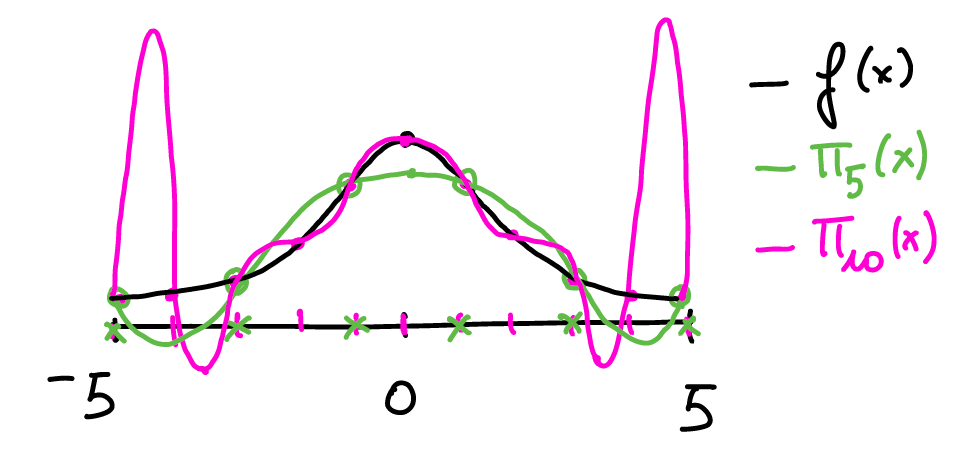
\includegraphics[width=0.5\textwidth]{pag39.PNG}
\end{center}
In figura vediamo l'andamento qualitativo dei grafici di $\prod_5(x)$ (6 nodi equispaziati) e di $\prod_{10}(x)$ (11 modi equispaziati): si vede chiaramente che verso gli estremi dell'intervallo pur infittendo il campionamento l'approssimazione peggiora.\\
Si può verificare che questo fenomeno persiste al crescere di $n$, in effetti (cosa che si può dimostrare teoricamente e comunque si vede "sperimentalmente") verso gli estremi si generano oscillazioni sempre più ampie col risultato che addirittura
\[
dist\left(\prod_n^{eq},\ \frac{1}{1+x^2}\right) = \underset{x \in [-5,5]}{max} \abs*{\prod_n^{eq}(x) - \frac{1}{1+x^2}}\underset{n \to \infty}{\longrightarrow} \infty
\] % TODO: ricontrollare
dove $eq$ indica interpolazione su nodi equispaziati.\\
Questo fenomeno di non convergenza (anzi, di \underline{divergenza}) mostra che la scelta di noti equispaziati non è appropriata per ricostruire una funzione per interpolazione con un unico polinomio di grado $\to \infty$
(la spiegazione teorica dell'esempio di Runge è molto profonda e necessita l'immersione del problema in campo complesso, essenzialmente le singolarità complesse di $f(z)$ che sono $\pm i$ (gli zeri complessi di $1+z^2, \ i^2 = -1$) si trovano "troppo vicine" all'intervallo in rapporto alla lunghezza dell'intervallo: in effetti ad esempio in $[-3,3]$ ci sarebbe convergenza usando nodi equispaziati (ma come già detto la teoria va ben oltre quello che si può fare in un corso base).\\
Concludiamo la lezione dicendo che ci sono \underline{2 strade} per risolvere
il problema della convergenza dell'interpolazione polinomiale, che esploreremo nelle prossime lezioni:
\begin{enumerate}
    \item usare \underline{distribuzioni speciali} dei nodi di campionamento
    \item cambiare tipo di interpolazione, passando dall'interpolazione con un unico polinomio di grado $\to \infty$, all'interpolazione \underline{polinomiale "a tratti"} in cui si usano polinomi di grado fissato su una suddivisione dell'intervallo in sottointervalli con ampiezza $\to 0$
\end{enumerate}

\end{document}

